% Options for packages loaded elsewhere
\PassOptionsToPackage{unicode}{hyperref}
\PassOptionsToPackage{hyphens}{url}
\PassOptionsToPackage{dvipsnames,svgnames,x11names}{xcolor}
%
\documentclass[
  10pt,
]{article}

\usepackage{amsmath,amssymb}
\usepackage{iftex}
\ifPDFTeX
  \usepackage[T1]{fontenc}
  \usepackage[utf8]{inputenc}
  \usepackage{textcomp} % provide euro and other symbols
\else % if luatex or xetex
  \usepackage{unicode-math}
  \defaultfontfeatures{Scale=MatchLowercase}
  \defaultfontfeatures[\rmfamily]{Ligatures=TeX,Scale=1}
\fi
\usepackage{lmodern}
\ifPDFTeX\else  
    % xetex/luatex font selection
\fi
% Use upquote if available, for straight quotes in verbatim environments
\IfFileExists{upquote.sty}{\usepackage{upquote}}{}
\IfFileExists{microtype.sty}{% use microtype if available
  \usepackage[]{microtype}
  \UseMicrotypeSet[protrusion]{basicmath} % disable protrusion for tt fonts
}{}
\makeatletter
\@ifundefined{KOMAClassName}{% if non-KOMA class
  \IfFileExists{parskip.sty}{%
    \usepackage{parskip}
  }{% else
    \setlength{\parindent}{0pt}
    \setlength{\parskip}{6pt plus 2pt minus 1pt}}
}{% if KOMA class
  \KOMAoptions{parskip=half}}
\makeatother
\usepackage{xcolor}
\setlength{\emergencystretch}{3em} % prevent overfull lines
\setcounter{secnumdepth}{-\maxdimen} % remove section numbering
% Make \paragraph and \subparagraph free-standing
\makeatletter
\ifx\paragraph\undefined\else
  \let\oldparagraph\paragraph
  \renewcommand{\paragraph}{
    \@ifstar
      \xxxParagraphStar
      \xxxParagraphNoStar
  }
  \newcommand{\xxxParagraphStar}[1]{\oldparagraph*{#1}\mbox{}}
  \newcommand{\xxxParagraphNoStar}[1]{\oldparagraph{#1}\mbox{}}
\fi
\ifx\subparagraph\undefined\else
  \let\oldsubparagraph\subparagraph
  \renewcommand{\subparagraph}{
    \@ifstar
      \xxxSubParagraphStar
      \xxxSubParagraphNoStar
  }
  \newcommand{\xxxSubParagraphStar}[1]{\oldsubparagraph*{#1}\mbox{}}
  \newcommand{\xxxSubParagraphNoStar}[1]{\oldsubparagraph{#1}\mbox{}}
\fi
\makeatother

\usepackage{color}
\usepackage{fancyvrb}
\newcommand{\VerbBar}{|}
\newcommand{\VERB}{\Verb[commandchars=\\\{\}]}
\DefineVerbatimEnvironment{Highlighting}{Verbatim}{commandchars=\\\{\}}
% Add ',fontsize=\small' for more characters per line
\usepackage{framed}
\definecolor{shadecolor}{RGB}{241,243,245}
\newenvironment{Shaded}{\begin{snugshade}}{\end{snugshade}}
\newcommand{\AlertTok}[1]{\textcolor[rgb]{0.68,0.00,0.00}{#1}}
\newcommand{\AnnotationTok}[1]{\textcolor[rgb]{0.37,0.37,0.37}{#1}}
\newcommand{\AttributeTok}[1]{\textcolor[rgb]{0.40,0.45,0.13}{#1}}
\newcommand{\BaseNTok}[1]{\textcolor[rgb]{0.68,0.00,0.00}{#1}}
\newcommand{\BuiltInTok}[1]{\textcolor[rgb]{0.00,0.23,0.31}{#1}}
\newcommand{\CharTok}[1]{\textcolor[rgb]{0.13,0.47,0.30}{#1}}
\newcommand{\CommentTok}[1]{\textcolor[rgb]{0.37,0.37,0.37}{#1}}
\newcommand{\CommentVarTok}[1]{\textcolor[rgb]{0.37,0.37,0.37}{\textit{#1}}}
\newcommand{\ConstantTok}[1]{\textcolor[rgb]{0.56,0.35,0.01}{#1}}
\newcommand{\ControlFlowTok}[1]{\textcolor[rgb]{0.00,0.23,0.31}{\textbf{#1}}}
\newcommand{\DataTypeTok}[1]{\textcolor[rgb]{0.68,0.00,0.00}{#1}}
\newcommand{\DecValTok}[1]{\textcolor[rgb]{0.68,0.00,0.00}{#1}}
\newcommand{\DocumentationTok}[1]{\textcolor[rgb]{0.37,0.37,0.37}{\textit{#1}}}
\newcommand{\ErrorTok}[1]{\textcolor[rgb]{0.68,0.00,0.00}{#1}}
\newcommand{\ExtensionTok}[1]{\textcolor[rgb]{0.00,0.23,0.31}{#1}}
\newcommand{\FloatTok}[1]{\textcolor[rgb]{0.68,0.00,0.00}{#1}}
\newcommand{\FunctionTok}[1]{\textcolor[rgb]{0.28,0.35,0.67}{#1}}
\newcommand{\ImportTok}[1]{\textcolor[rgb]{0.00,0.46,0.62}{#1}}
\newcommand{\InformationTok}[1]{\textcolor[rgb]{0.37,0.37,0.37}{#1}}
\newcommand{\KeywordTok}[1]{\textcolor[rgb]{0.00,0.23,0.31}{\textbf{#1}}}
\newcommand{\NormalTok}[1]{\textcolor[rgb]{0.00,0.23,0.31}{#1}}
\newcommand{\OperatorTok}[1]{\textcolor[rgb]{0.37,0.37,0.37}{#1}}
\newcommand{\OtherTok}[1]{\textcolor[rgb]{0.00,0.23,0.31}{#1}}
\newcommand{\PreprocessorTok}[1]{\textcolor[rgb]{0.68,0.00,0.00}{#1}}
\newcommand{\RegionMarkerTok}[1]{\textcolor[rgb]{0.00,0.23,0.31}{#1}}
\newcommand{\SpecialCharTok}[1]{\textcolor[rgb]{0.37,0.37,0.37}{#1}}
\newcommand{\SpecialStringTok}[1]{\textcolor[rgb]{0.13,0.47,0.30}{#1}}
\newcommand{\StringTok}[1]{\textcolor[rgb]{0.13,0.47,0.30}{#1}}
\newcommand{\VariableTok}[1]{\textcolor[rgb]{0.07,0.07,0.07}{#1}}
\newcommand{\VerbatimStringTok}[1]{\textcolor[rgb]{0.13,0.47,0.30}{#1}}
\newcommand{\WarningTok}[1]{\textcolor[rgb]{0.37,0.37,0.37}{\textit{#1}}}

\providecommand{\tightlist}{%
  \setlength{\itemsep}{0pt}\setlength{\parskip}{0pt}}\usepackage{longtable,booktabs,array}
\usepackage{calc} % for calculating minipage widths
% Correct order of tables after \paragraph or \subparagraph
\usepackage{etoolbox}
\makeatletter
\patchcmd\longtable{\par}{\if@noskipsec\mbox{}\fi\par}{}{}
\makeatother
% Allow footnotes in longtable head/foot
\IfFileExists{footnotehyper.sty}{\usepackage{footnotehyper}}{\usepackage{footnote}}
\makesavenoteenv{longtable}
\usepackage{graphicx}
\makeatletter
\def\maxwidth{\ifdim\Gin@nat@width>\linewidth\linewidth\else\Gin@nat@width\fi}
\def\maxheight{\ifdim\Gin@nat@height>\textheight\textheight\else\Gin@nat@height\fi}
\makeatother
% Scale images if necessary, so that they will not overflow the page
% margins by default, and it is still possible to overwrite the defaults
% using explicit options in \includegraphics[width, height, ...]{}
\setkeys{Gin}{width=\maxwidth,height=\maxheight,keepaspectratio}
% Set default figure placement to htbp
\makeatletter
\def\fps@figure{htbp}
\makeatother

\usepackage{booktabs}
\usepackage{longtable}
\usepackage{array}
\usepackage{multirow}
\usepackage{wrapfig}
\usepackage{float}
\usepackage{colortbl}
\usepackage{pdflscape}
\usepackage{tabu}
\usepackage{threeparttable}
\usepackage{threeparttablex}
\usepackage[normalem]{ulem}
\usepackage{makecell}
\usepackage{xcolor}
\usepackage{geometry}
\geometry{top=1in, bottom=1in, left=1in, right=1in}
\usepackage{listings}
\lstset{ breaklines=true, breakatwhitespace=true, basicstyle=\ttfamily\small, frame=single, tabsize=2, xleftmargin=0.5cm, xrightmargin=0.5cm}
\usepackage{setspace}
\setstretch{1.15}
\usepackage{parskip}
\setlength{\parskip}{0.5em}
\setlength{\parindent}{0em}
\setlength{\emergencystretch}{3em}
\usepackage{placeins}
\makeatletter
\@ifpackageloaded{caption}{}{\usepackage{caption}}
\AtBeginDocument{%
\ifdefined\contentsname
  \renewcommand*\contentsname{Table of contents}
\else
  \newcommand\contentsname{Table of contents}
\fi
\ifdefined\listfigurename
  \renewcommand*\listfigurename{List of Figures}
\else
  \newcommand\listfigurename{List of Figures}
\fi
\ifdefined\listtablename
  \renewcommand*\listtablename{List of Tables}
\else
  \newcommand\listtablename{List of Tables}
\fi
\ifdefined\figurename
  \renewcommand*\figurename{Figure}
\else
  \newcommand\figurename{Figure}
\fi
\ifdefined\tablename
  \renewcommand*\tablename{Table}
\else
  \newcommand\tablename{Table}
\fi
}
\@ifpackageloaded{float}{}{\usepackage{float}}
\floatstyle{ruled}
\@ifundefined{c@chapter}{\newfloat{codelisting}{h}{lop}}{\newfloat{codelisting}{h}{lop}[chapter]}
\floatname{codelisting}{Listing}
\newcommand*\listoflistings{\listof{codelisting}{List of Listings}}
\makeatother
\makeatletter
\makeatother
\makeatletter
\@ifpackageloaded{caption}{}{\usepackage{caption}}
\@ifpackageloaded{subcaption}{}{\usepackage{subcaption}}
\makeatother

\ifLuaTeX
  \usepackage{selnolig}  % disable illegal ligatures
\fi
\usepackage{bookmark}

\IfFileExists{xurl.sty}{\usepackage{xurl}}{} % add URL line breaks if available
\urlstyle{same} % disable monospaced font for URLs
\hypersetup{
  pdftitle={Untitled},
  colorlinks=true,
  linkcolor={blue},
  filecolor={Maroon},
  citecolor={Blue},
  urlcolor={Blue},
  pdfcreator={LaTeX via pandoc}}


\title{Untitled}
\author{}
\date{}

\begin{document}
\maketitle


l

\begin{verbatim}
Installing package into 'C:/Users/vasud/AppData/Local/R/win-library/4.4'
(as 'lib' is unspecified)
\end{verbatim}

\begin{verbatim}
package 'ggthemes' successfully unpacked and MD5 sums checked

The downloaded binary packages are in
    C:\Users\vasud\AppData\Local\Temp\RtmpMFYmLY\downloaded_packages
\end{verbatim}

\begin{verbatim}
-- Attaching core tidyverse packages ------------------------ tidyverse 2.0.0 --
v dplyr     1.1.4     v readr     2.1.5
v forcats   1.0.0     v stringr   1.5.1
v ggplot2   3.5.1     v tibble    3.2.1
v lubridate 1.9.4     v tidyr     1.3.1
v purrr     1.0.2     
-- Conflicts ------------------------------------------ tidyverse_conflicts() --
x dplyr::filter() masks stats::filter()
x dplyr::lag()    masks stats::lag()
i Use the conflicted package (<http://conflicted.r-lib.org/>) to force all conflicts to become errors

Attaching package: 'data.table'


The following objects are masked from 'package:lubridate':

    hour, isoweek, mday, minute, month, quarter, second, wday, week,
    yday, year


The following objects are masked from 'package:dplyr':

    between, first, last


The following object is masked from 'package:purrr':

    transpose



Attaching package: 'janitor'


The following objects are masked from 'package:stats':

    chisq.test, fisher.test



Attaching package: 'jsonlite'


The following object is masked from 'package:purrr':

    flatten



Attaching package: 'plotly'


The following object is masked from 'package:httr':

    config


The following object is masked from 'package:ggplot2':

    last_plot


The following object is masked from 'package:stats':

    filter


The following object is masked from 'package:graphics':

    layout


corrplot 0.95 loaded

Loading required package: zoo


Attaching package: 'zoo'


The following objects are masked from 'package:data.table':

    yearmon, yearqtr


The following objects are masked from 'package:base':

    as.Date, as.Date.numeric


Loading required package: lattice


Attaching package: 'caret'


The following object is masked from 'package:httr':

    progress


The following object is masked from 'package:purrr':

    lift



Attaching package: 'MASS'


The following object is masked from 'package:plotly':

    select


The following object is masked from 'package:dplyr':

    select


Loading required package: Matrix


Attaching package: 'Matrix'


The following objects are masked from 'package:tidyr':

    expand, pack, unpack


Registered S3 method overwritten by 'quantmod':
  method            from
  as.zoo.data.frame zoo 


Attaching package: 'forecast'


The following object is masked from 'package:ggpubr':

    gghistogram


Loading required package: car

Loading required package: carData


Attaching package: 'car'


The following object is masked from 'package:dplyr':

    recode


The following object is masked from 'package:purrr':

    some


Loading required package: survival


Attaching package: 'survival'


The following object is masked from 'package:caret':

    cluster


Loading required package: StanHeaders


rstan version 2.32.6 (Stan version 2.32.2)


For execution on a local, multicore CPU with excess RAM we recommend calling
options(mc.cores = parallel::detectCores()).
To avoid recompilation of unchanged Stan programs, we recommend calling
rstan_options(auto_write = TRUE)
For within-chain threading using `reduce_sum()` or `map_rect()` Stan functions,
change `threads_per_chain` option:
rstan_options(threads_per_chain = 1)


Do not specify '-march=native' in 'LOCAL_CPPFLAGS' or a Makevars file


Attaching package: 'rstan'


The following object is masked from 'package:tidyr':

    extract


Loading required package: Rcpp

Loading 'brms' package (version 2.22.0). Useful instructions
can be found by typing help('brms'). A more detailed introduction
to the package is available through vignette('brms_overview').


Attaching package: 'brms'


The following object is masked from 'package:rstan':

    loo


The following object is masked from 'package:survival':

    kidney


The following object is masked from 'package:forecast':

    ma


The following object is masked from 'package:lme4':

    ngrps


The following object is masked from 'package:stats':

    ar



Attaching package: 'coda'


The following object is masked from 'package:rstan':

    traceplot


************
Welcome to BayesFactor 0.9.12-4.7. If you have questions, please contact Richard Morey (richarddmorey@gmail.com).

Type BFManual() to open the manual.
************

Loading required package: antitrust


Attaching package: 'antitrust'


The following object is masked from 'package:car':

    logit


The following object is masked from 'package:forecast':

    CV



Attaching package: 'trade'


The following object is masked from 'package:antitrust':

    sim



Attaching package: 'kableExtra'


The following object is masked from 'package:dplyr':

    group_rows



Attaching package: 'officer'


The following object is masked from 'package:readxl':

    read_xlsx



Attaching package: 'xgboost'


The following object is masked from 'package:plotly':

    slice


The following object is masked from 'package:dplyr':

    slice


Loaded glmnet 4.1-8

-- Attaching packages -------------------------------------- tidymodels 1.2.0 --

v broom        1.0.7     v rsample      1.2.1
v dials        1.3.0     v tune         1.2.1
v infer        1.0.7     v workflows    1.1.4
v modeldata    1.4.0     v workflowsets 1.1.0
v parsnip      1.2.1     v yardstick    1.3.1
v recipes      1.1.0     

-- Conflicts ----------------------------------------- tidymodels_conflicts() --
x yardstick::accuracy()    masks forecast::accuracy()
x data.table::between()    masks dplyr::between()
x scales::discard()        masks purrr::discard()
x Matrix::expand()         masks tidyr::expand()
x rstan::extract()         masks tidyr::extract()
x plotly::filter()         masks dplyr::filter(), stats::filter()
x data.table::first()      masks dplyr::first()
x recipes::fixed()         masks stringr::fixed()
x jsonlite::flatten()      masks purrr::flatten()
x kableExtra::group_rows() masks dplyr::group_rows()
x dplyr::lag()             masks stats::lag()
x data.table::last()       masks dplyr::last()
x caret::lift()            masks purrr::lift()
x dials::mixture()         masks brms::mixture()
x Matrix::pack()           masks tidyr::pack()
x rsample::populate()      masks Rcpp::populate()
x yardstick::precision()   masks caret::precision()
x yardstick::recall()      masks caret::recall()
x car::recode()            masks dplyr::recode()
x MASS::select()           masks plotly::select(), dplyr::select()
x yardstick::sensitivity() masks caret::sensitivity()
x xgboost::slice()         masks plotly::slice(), dplyr::slice()
x car::some()              masks purrr::some()
x yardstick::spec()        masks readr::spec()
x yardstick::specificity() masks caret::specificity()
x recipes::step()          masks stats::step()
x data.table::transpose()  masks purrr::transpose()
x Matrix::unpack()         masks tidyr::unpack()
x recipes::update()        masks Matrix::update(), stats::update()
* Search for functions across packages at https://www.tidymodels.org/find/
\end{verbatim}

\begin{verbatim}
[1] "All required libraries are loaded!"
\end{verbatim}

\begin{verbatim}
Registered S3 method overwritten by 'GGally':
  method from   
  +.gg   ggplot2
\end{verbatim}

\begin{verbatim}

Attaching package: 'dataMaid'
\end{verbatim}

\begin{verbatim}
The following object is masked from 'package:recipes':

    check
\end{verbatim}

\begin{verbatim}
The following object is masked from 'package:infer':

    visualize
\end{verbatim}

\begin{verbatim}
The following object is masked from 'package:rmarkdown':

    render
\end{verbatim}

\begin{verbatim}
The following object is masked from 'package:lme4':

    isSingular
\end{verbatim}

\begin{verbatim}
The following object is masked from 'package:dplyr':

    summarize
\end{verbatim}

\begin{verbatim}
Rows: 23977 Columns: 6
-- Column specification --------------------------------------------------------
Delimiter: ","
chr (1): CountryName
dbl (4): Year, Value of global merchandise exports as a share of GDP, GDP pe...
lgl (1): World regions according to OWID

i Use `spec()` to retrieve the full column specification for this data.
i Specify the column types or set `show_col_types = FALSE` to quiet this message.
\end{verbatim}

\begin{Shaded}
\begin{Highlighting}[]
\FunctionTok{colnames}\NormalTok{(Trade)}
\end{Highlighting}
\end{Shaded}

\begin{verbatim}
[1] "CountryName"                                          
[2] "Year"                                                 
[3] "Value of global merchandise exports as a share of GDP"
[4] "GDP per capita"                                       
[5] "Population (historical)"                              
[6] "World regions according to OWID"                      
\end{verbatim}

\begin{Shaded}
\begin{Highlighting}[]
\FunctionTok{print}\NormalTok{(}\FunctionTok{summary}\NormalTok{(Trade))}
\end{Highlighting}
\end{Shaded}

\begin{verbatim}
 CountryName             Year     
 Length:23977       Min.   :   1  
 Class :character   1st Qu.:1877  
 Mode  :character   Median :1961  
                    Mean   :1894  
                    3rd Qu.:1993  
                    Max.   :2022  
                                  
 Value of global merchandise exports as a share of GDP GDP per capita  
 Min.   :  0.00                                        Min.   :   295  
 1st Qu.: 11.16                                        1st Qu.:  1470  
 Median : 19.03                                        Median :  2618  
 Mean   : 25.59                                        Mean   :  6870  
 3rd Qu.: 31.36                                        3rd Qu.:  7232  
 Max.   :779.76                                        Max.   :160051  
 NA's   :10169                                         NA's   :2391    
 Population (historical) World regions according to OWID
 Min.   :8.821e+03       Mode:logical                   
 1st Qu.:1.991e+06       NA's:23977                     
 Median :5.704e+06                                      
 Mean   :5.799e+07                                      
 3rd Qu.:1.921e+07                                      
 Max.   :8.021e+09                                      
 NA's   :4953                                           
\end{verbatim}

\begin{Shaded}
\begin{Highlighting}[]
\FunctionTok{colnames}\NormalTok{(CW\_Data)}
\end{Highlighting}
\end{Shaded}

\begin{verbatim}
[1] "CountryName"                 "Year"                       
[3] "CurrentYearTotalTradeValue"  "PreviousYearTotalTradeValue"
[5] "GrowthPercentage"            "AverageGrowthPercentage"    
\end{verbatim}

\begin{Shaded}
\begin{Highlighting}[]
\FunctionTok{print}\NormalTok{(}\FunctionTok{summary}\NormalTok{(CW\_Data))}
\end{Highlighting}
\end{Shaded}

\begin{verbatim}
 CountryName             Year      CurrentYearTotalTradeValue
 Length:4554        Min.   :1989   Min.   :3.000e+00         
 Class :character   1st Qu.:2000   1st Qu.:1.634e+06         
 Mode  :character   Median :2007   Median :1.361e+07         
                    Mean   :2007   Mean   :1.623e+08         
                    3rd Qu.:2014   3rd Qu.:1.072e+08         
                    Max.   :2021   Max.   :5.181e+09         
 PreviousYearTotalTradeValue GrowthPercentage   AverageGrowthPercentage
 Min.   :3.000e+00           Min.   : -89.230   Min.   :-34.43         
 1st Qu.:1.528e+06           1st Qu.:  -4.685   1st Qu.:  5.81         
 Median :1.274e+07           Median :   6.830   Median :  8.31         
 Mean   :1.544e+08           Mean   :  12.361   Mean   : 12.36         
 3rd Qu.:9.970e+07           3rd Qu.:  18.538   3rd Qu.: 11.73         
 Max.   :4.997e+09           Max.   :5511.730   Max.   :478.50         
\end{verbatim}

\begin{Shaded}
\begin{Highlighting}[]
\NormalTok{AnnVal }\OtherTok{\textless{}{-}} \FunctionTok{read.csv}\NormalTok{(}\StringTok{"C:/Users/vasud/OneDrive/Desktop/U{-}M {-} ALL/STATS 506/Final Project Data/KAGGLE/archive/AnnualValue.csv"}\NormalTok{)}
\end{Highlighting}
\end{Shaded}

\begin{Shaded}
\begin{Highlighting}[]
\NormalTok{merged\_data\_full }\OtherTok{\textless{}{-}} \FunctionTok{left\_join}\NormalTok{(Trade, CW\_Data, }\AttributeTok{by =} \FunctionTok{c}\NormalTok{(}\StringTok{"CountryName"} \OtherTok{=} \StringTok{"CountryName"}\NormalTok{, }\StringTok{"Year"} \OtherTok{=} \StringTok{"Year"}\NormalTok{))}
\NormalTok{merged\_data\_full2 }\OtherTok{\textless{}{-}} \FunctionTok{left\_join}\NormalTok{(merged\_data\_full, AnnVal, }\AttributeTok{by =} \FunctionTok{c}\NormalTok{(}\StringTok{"CountryName"} \OtherTok{=} \StringTok{"CountryName"}\NormalTok{, }\StringTok{"Year"} \OtherTok{=} \StringTok{"Year"}\NormalTok{))}
\end{Highlighting}
\end{Shaded}

\begin{Shaded}
\begin{Highlighting}[]
\FunctionTok{colnames}\NormalTok{(merged\_data\_full2)}
\end{Highlighting}
\end{Shaded}

\begin{verbatim}
 [1] "CountryName"                                          
 [2] "Year"                                                 
 [3] "Value of global merchandise exports as a share of GDP"
 [4] "GDP per capita"                                       
 [5] "Population (historical)"                              
 [6] "World regions according to OWID"                      
 [7] "CurrentYearTotalTradeValue"                           
 [8] "PreviousYearTotalTradeValue"                          
 [9] "GrowthPercentage"                                     
[10] "AverageGrowthPercentage"                              
[11] "AnnualTradeValue"                                     
\end{verbatim}

\begin{Shaded}
\begin{Highlighting}[]
\NormalTok{merged\_data\_full2 }\OtherTok{\textless{}{-}}\NormalTok{ merged\_data\_full2[, }\SpecialCharTok{!}\NormalTok{(}\FunctionTok{names}\NormalTok{(merged\_data\_full2) }\SpecialCharTok{\%in\%} \FunctionTok{c}\NormalTok{(}\StringTok{"World regions according to OWID"}\NormalTok{))]}
\FunctionTok{colnames}\NormalTok{(merged\_data\_full2)}
\end{Highlighting}
\end{Shaded}

\begin{verbatim}
 [1] "CountryName"                                          
 [2] "Year"                                                 
 [3] "Value of global merchandise exports as a share of GDP"
 [4] "GDP per capita"                                       
 [5] "Population (historical)"                              
 [6] "CurrentYearTotalTradeValue"                           
 [7] "PreviousYearTotalTradeValue"                          
 [8] "GrowthPercentage"                                     
 [9] "AverageGrowthPercentage"                              
[10] "AnnualTradeValue"                                     
\end{verbatim}

\begin{Shaded}
\begin{Highlighting}[]
\NormalTok{TradeData }\OtherTok{\textless{}{-}}\NormalTok{ merged\_data\_full2}
\FunctionTok{colnames}\NormalTok{(TradeData)}
\end{Highlighting}
\end{Shaded}

\begin{verbatim}
 [1] "CountryName"                                          
 [2] "Year"                                                 
 [3] "Value of global merchandise exports as a share of GDP"
 [4] "GDP per capita"                                       
 [5] "Population (historical)"                              
 [6] "CurrentYearTotalTradeValue"                           
 [7] "PreviousYearTotalTradeValue"                          
 [8] "GrowthPercentage"                                     
 [9] "AverageGrowthPercentage"                              
[10] "AnnualTradeValue"                                     
\end{verbatim}

\begin{Shaded}
\begin{Highlighting}[]
\FunctionTok{summary}\NormalTok{(TradeData)}
\end{Highlighting}
\end{Shaded}

\begin{verbatim}
 CountryName             Year     
 Length:23977       Min.   :   1  
 Class :character   1st Qu.:1877  
 Mode  :character   Median :1961  
                    Mean   :1894  
                    3rd Qu.:1993  
                    Max.   :2022  
                                  
 Value of global merchandise exports as a share of GDP GDP per capita  
 Min.   :  0.00                                        Min.   :   295  
 1st Qu.: 11.16                                        1st Qu.:  1470  
 Median : 19.03                                        Median :  2618  
 Mean   : 25.59                                        Mean   :  6870  
 3rd Qu.: 31.36                                        3rd Qu.:  7232  
 Max.   :779.76                                        Max.   :160051  
 NA's   :10169                                         NA's   :2391    
 Population (historical) CurrentYearTotalTradeValue PreviousYearTotalTradeValue
 Min.   :8.821e+03       Min.   :1.250e+02          Min.   :1.950e+02          
 1st Qu.:1.991e+06       1st Qu.:2.674e+06          1st Qu.:2.480e+06          
 Median :5.704e+06       Median :1.708e+07          Median :1.587e+07          
 Mean   :5.799e+07       Mean   :1.571e+08          Mean   :1.497e+08          
 3rd Qu.:1.921e+07       3rd Qu.:1.134e+08          3rd Qu.:1.072e+08          
 Max.   :8.021e+09       Max.   :5.181e+09          Max.   :4.997e+09          
 NA's   :4953            NA's   :20197              NA's   :20197              
 GrowthPercentage  AverageGrowthPercentage AnnualTradeValue   
 Min.   : -86.12   Min.   :-34.43          Min.   :1.250e+02  
 1st Qu.:  -3.95   1st Qu.:  5.81          1st Qu.:2.329e+06  
 Median :   7.06   Median :  8.42          Median :1.465e+07  
 Mean   :  10.83   Mean   : 10.61          Mean   :1.490e+08  
 3rd Qu.:  18.46   3rd Qu.: 11.57          3rd Qu.:1.031e+08  
 Max.   :1951.04   Max.   :292.12          Max.   :5.181e+09  
 NA's   :20197     NA's   :20197           NA's   :19947      
\end{verbatim}

\begin{Shaded}
\begin{Highlighting}[]
\FunctionTok{summary}\NormalTok{(TradeData}\SpecialCharTok{$}\NormalTok{AnnualTradeValue)}
\end{Highlighting}
\end{Shaded}

\begin{verbatim}
     Min.   1st Qu.    Median      Mean   3rd Qu.      Max.      NA's 
1.250e+02 2.329e+06 1.465e+07 1.490e+08 1.031e+08 5.181e+09     19947 
\end{verbatim}

\begin{Shaded}
\begin{Highlighting}[]
\NormalTok{TradeData\_clean }\OtherTok{\textless{}{-}} \FunctionTok{na.omit}\NormalTok{(TradeData)}
\end{Highlighting}
\end{Shaded}

\subsubsection{Cleaning and preparing the
data}\label{cleaning-and-preparing-the-data}

\begin{Shaded}
\begin{Highlighting}[]
\CommentTok{\# Remove rows with NA values in specified columns}
\NormalTok{TradeData }\OtherTok{\textless{}{-}}\NormalTok{ TradeData }\SpecialCharTok{\%\textgreater{}\%}
  \FunctionTok{filter}\NormalTok{(}\SpecialCharTok{!}\FunctionTok{is.na}\NormalTok{(}\StringTok{\textasciigrave{}}\AttributeTok{GDP per capita}\StringTok{\textasciigrave{}}\NormalTok{) }\SpecialCharTok{\&} 
         \SpecialCharTok{!}\FunctionTok{is.na}\NormalTok{(}\StringTok{\textasciigrave{}}\AttributeTok{Value of global merchandise exports as a share of GDP}\StringTok{\textasciigrave{}}\NormalTok{) }\SpecialCharTok{\&} 
         \SpecialCharTok{!}\FunctionTok{is.na}\NormalTok{(GrowthPercentage))}
\end{Highlighting}
\end{Shaded}

\begin{Shaded}
\begin{Highlighting}[]
\FunctionTok{summary}\NormalTok{(TradeData)}
\end{Highlighting}
\end{Shaded}

\begin{verbatim}
 CountryName             Year     
 Length:2680        Min.   :1989  
 Class :character   1st Qu.:1998  
 Mode  :character   Median :2004  
                    Mean   :2003  
                    3rd Qu.:2009  
                    Max.   :2014  
 Value of global merchandise exports as a share of GDP GDP per capita  
 Min.   :  1.441                                       Min.   :   561  
 1st Qu.: 16.718                                       1st Qu.:  4333  
 Median : 25.572                                       Median : 10694  
 Mean   : 31.336                                       Mean   : 16165  
 3rd Qu.: 40.247                                       3rd Qu.: 24513  
 Max.   :183.905                                       Max.   :157713  
 Population (historical) CurrentYearTotalTradeValue PreviousYearTotalTradeValue
 Min.   :6.830e+04       Min.   :5.177e+03          Min.   :5.177e+03          
 1st Qu.:3.796e+06       1st Qu.:3.210e+06          1st Qu.:2.966e+06          
 Median :1.008e+07       Median :1.968e+07          Median :1.769e+07          
 Mean   :4.799e+07       Mean   :1.482e+08          Mean   :1.386e+08          
 3rd Qu.:2.922e+07       3rd Qu.:1.161e+08          3rd Qu.:1.067e+08          
 Max.   :1.388e+09       Max.   :4.685e+09          Max.   :4.418e+09          
 GrowthPercentage   AverageGrowthPercentage AnnualTradeValue   
 Min.   : -84.300   Min.   :-34.43          Min.   :5.177e+03  
 1st Qu.:  -1.093   1st Qu.:  5.91          1st Qu.:3.210e+06  
 Median :   9.205   Median :  8.50          Median :1.968e+07  
 Mean   :  12.557   Mean   : 10.33          Mean   :1.482e+08  
 3rd Qu.:  20.270   3rd Qu.: 11.70          3rd Qu.:1.161e+08  
 Max.   :1951.040   Max.   : 88.73          Max.   :4.685e+09  
\end{verbatim}

\begin{Shaded}
\begin{Highlighting}[]
\FunctionTok{library}\NormalTok{(car) }

\CommentTok{\# Compute VIF}
\FunctionTok{vif}\NormalTok{(}\FunctionTok{lm}\NormalTok{(GrowthPercentage }\SpecialCharTok{\textasciitilde{}} \StringTok{\textasciigrave{}}\AttributeTok{GDP per capita}\StringTok{\textasciigrave{}} \SpecialCharTok{+} \StringTok{\textasciigrave{}}\AttributeTok{Value of global merchandise exports as a share of GDP}\StringTok{\textasciigrave{}}\NormalTok{, }\AttributeTok{data =}\NormalTok{ TradeData))}
\end{Highlighting}
\end{Shaded}

\begin{verbatim}
                                       `GDP per capita` 
                                               1.103906 
`Value of global merchandise exports as a share of GDP` 
                                               1.103906 
\end{verbatim}

\begin{Shaded}
\begin{Highlighting}[]
\CommentTok{\# Check correlations between predictors}
\FunctionTok{cor}\NormalTok{(TradeData[, }\FunctionTok{c}\NormalTok{(}\StringTok{"GDP per capita"}\NormalTok{, }\StringTok{"Value of global merchandise exports as a share of GDP"}\NormalTok{, }\StringTok{"AnnualTradeValue"}\NormalTok{)])}
\end{Highlighting}
\end{Shaded}

\begin{verbatim}
                                                      GDP per capita
GDP per capita                                             1.0000000
Value of global merchandise exports as a share of GDP      0.3067997
AnnualTradeValue                                           0.3809786
                                                      Value of global merchandise exports as a share of GDP
GDP per capita                                                                                   0.30679970
Value of global merchandise exports as a share of GDP                                            1.00000000
AnnualTradeValue                                                                                 0.04389992
                                                      AnnualTradeValue
GDP per capita                                              0.38097857
Value of global merchandise exports as a share of GDP       0.04389992
AnnualTradeValue                                            1.00000000
\end{verbatim}

\begin{enumerate}
\def\labelenumi{\arabic{enumi}.}
\item
  \textbf{GDP per capita and Annual Trade Value}: The correlation is
  \textbf{0.38}, indicating a moderate positive relationship. This
  suggests that as GDP per capita increases, the annual trade value
  tends to increase as well, though not strongly.
\item
  \textbf{Value of Global Merchandise Exports as a Share of GDP and
  Annual Trade Value}: The correlation is quite \textbf{low} at
  \textbf{0.04}, indicating almost no linear relationship between these
  two variables. This implies that the share of merchandise exports as a
  portion of GDP is not strongly related to the total annual trade
  value.
\item
  \textbf{GDP per capita and Value of Global Merchandise Exports as a
  Share of GDP}: The correlation here is \textbf{0.31}, suggesting a
  weak to moderate positive relationship. This could indicate that
  richer countries (higher GDP per capita) tend to have a somewhat
  higher share of exports relative to GDP, but the relationship is not
  particularly strong.
\end{enumerate}

\begin{Shaded}
\begin{Highlighting}[]
\CommentTok{\# Run model with all predictors}
\NormalTok{lm\_full }\OtherTok{\textless{}{-}} \FunctionTok{lm}\NormalTok{(GrowthPercentage }\SpecialCharTok{\textasciitilde{}} \StringTok{\textasciigrave{}}\AttributeTok{GDP per capita}\StringTok{\textasciigrave{}} \SpecialCharTok{+} \StringTok{\textasciigrave{}}\AttributeTok{Value of global merchandise exports as a share of GDP}\StringTok{\textasciigrave{}} \SpecialCharTok{+}\NormalTok{ AnnualTradeValue, }\AttributeTok{data =}\NormalTok{ TradeData)}

\CommentTok{\# Compute VIF}
\FunctionTok{vif}\NormalTok{(lm\_full)}
\end{Highlighting}
\end{Shaded}

\begin{verbatim}
                                       `GDP per capita` 
                                               1.297775 
`Value of global merchandise exports as a share of GDP` 
                                               1.111552 
                                       AnnualTradeValue 
                                               1.177891 
\end{verbatim}

\begin{Shaded}
\begin{Highlighting}[]
\CommentTok{\# Fit a reduced model (with three variables for VIF)}
\NormalTok{lm\_reduced }\OtherTok{\textless{}{-}} \FunctionTok{lm}\NormalTok{(GrowthPercentage }\SpecialCharTok{\textasciitilde{}} \StringTok{\textasciigrave{}}\AttributeTok{GDP per capita}\StringTok{\textasciigrave{}} \SpecialCharTok{+} \StringTok{\textasciigrave{}}\AttributeTok{Value of global merchandise exports as a share of GDP}\StringTok{\textasciigrave{}} \SpecialCharTok{+}\NormalTok{ AnnualTradeValue, }\AttributeTok{data =}\NormalTok{ TradeData)}

\CommentTok{\# Compute VIF}
\FunctionTok{vif}\NormalTok{(lm\_reduced)}
\end{Highlighting}
\end{Shaded}

\begin{verbatim}
                                       `GDP per capita` 
                                               1.297775 
`Value of global merchandise exports as a share of GDP` 
                                               1.111552 
                                       AnnualTradeValue 
                                               1.177891 
\end{verbatim}

\begin{Shaded}
\begin{Highlighting}[]
\FunctionTok{library}\NormalTok{(mice)}
\end{Highlighting}
\end{Shaded}

\begin{verbatim}

Attaching package: 'mice'
\end{verbatim}

\begin{verbatim}
The following object is masked from 'package:stats':

    filter
\end{verbatim}

\begin{verbatim}
The following objects are masked from 'package:base':

    cbind, rbind
\end{verbatim}

\begin{Shaded}
\begin{Highlighting}[]
\NormalTok{imputed\_data }\OtherTok{\textless{}{-}} \FunctionTok{mice}\NormalTok{(TradeData, }\AttributeTok{m =} \DecValTok{1}\NormalTok{, }\AttributeTok{method =} \StringTok{\textquotesingle{}pmm\textquotesingle{}}\NormalTok{, }\AttributeTok{maxit =} \DecValTok{10}\NormalTok{, }\AttributeTok{seed =} \DecValTok{123}\NormalTok{)}
\end{Highlighting}
\end{Shaded}

\begin{verbatim}

 iter imp variable
  1   1
  2   1
  3   1
  4   1
  5   1
  6   1
  7   1
  8   1
  9   1
  10   1
\end{verbatim}

\begin{verbatim}
Warning: Number of logged events: 2
\end{verbatim}

\begin{Shaded}
\begin{Highlighting}[]
\NormalTok{TradeData\_imputed }\OtherTok{\textless{}{-}} \FunctionTok{complete}\NormalTok{(imputed\_data)}

\CommentTok{\# Perform PCA including the new variable}
\NormalTok{pca }\OtherTok{\textless{}{-}} \FunctionTok{prcomp}\NormalTok{(TradeData\_imputed[, }\FunctionTok{c}\NormalTok{(}\StringTok{"GDP per capita"}\NormalTok{, }\StringTok{"Value of global merchandise exports as a share of GDP"}\NormalTok{, }\StringTok{"AnnualTradeValue"}\NormalTok{)], }\AttributeTok{scale. =} \ConstantTok{TRUE}\NormalTok{)}

\CommentTok{\# Get the first principal component}
\NormalTok{TradeData\_imputed}\SpecialCharTok{$}\NormalTok{PCA1 }\OtherTok{\textless{}{-}}\NormalTok{ pca}\SpecialCharTok{$}\NormalTok{x[, }\DecValTok{1}\NormalTok{]}

\CommentTok{\# Use the first principal component in the regression model}
\NormalTok{model\_pca }\OtherTok{\textless{}{-}} \FunctionTok{lm}\NormalTok{(GrowthPercentage }\SpecialCharTok{\textasciitilde{}}\NormalTok{ PCA1, }\AttributeTok{data =}\NormalTok{ TradeData\_imputed)}
\FunctionTok{summary}\NormalTok{(model\_pca)}
\end{Highlighting}
\end{Shaded}

\begin{verbatim}

Call:
lm(formula = GrowthPercentage ~ PCA1, data = TradeData_imputed)

Residuals:
    Min      1Q  Median      3Q     Max 
 -97.77  -13.66   -3.26    7.78 1938.23 

Coefficients:
            Estimate Std. Error t value Pr(>|t|)    
(Intercept)  12.5574     0.9813  12.797   <2e-16 ***
PCA1         -0.8157     0.7984  -1.022    0.307    
---
Signif. codes:  0 '***' 0.001 '**' 0.01 '*' 0.05 '.' 0.1 ' ' 1

Residual standard error: 50.8 on 2678 degrees of freedom
Multiple R-squared:  0.0003896, Adjusted R-squared:  1.635e-05 
F-statistic: 1.044 on 1 and 2678 DF,  p-value: 0.307
\end{verbatim}

\begin{Shaded}
\begin{Highlighting}[]
\CommentTok{\# Run the regression again with the new variable included}
\NormalTok{model }\OtherTok{\textless{}{-}} \FunctionTok{lm}\NormalTok{(GrowthPercentage }\SpecialCharTok{\textasciitilde{}} \StringTok{\textasciigrave{}}\AttributeTok{GDP per capita}\StringTok{\textasciigrave{}} \SpecialCharTok{+} \StringTok{\textasciigrave{}}\AttributeTok{Value of global merchandise exports as a share of GDP}\StringTok{\textasciigrave{}} \SpecialCharTok{+}\NormalTok{ AnnualTradeValue, }\AttributeTok{data =}\NormalTok{ TradeData\_imputed)}
\FunctionTok{summary}\NormalTok{(model)}
\end{Highlighting}
\end{Shaded}

\begin{verbatim}

Call:
lm(formula = GrowthPercentage ~ `GDP per capita` + `Value of global merchandise exports as a share of GDP` + 
    AnnualTradeValue, data = TradeData_imputed)

Residuals:
    Min      1Q  Median      3Q     Max 
 -96.41  -13.62   -3.18    7.89 1938.90 

Coefficients:
                                                          Estimate Std. Error
(Intercept)                                              1.213e+01  1.787e+00
`GDP per capita`                                        -1.058e-04  6.852e-05
`Value of global merchandise exports as a share of GDP`  7.814e-02  4.616e-02
AnnualTradeValue                                        -2.124e-09  2.903e-09
                                                        t value Pr(>|t|)    
(Intercept)                                               6.789 1.38e-11 ***
`GDP per capita`                                         -1.545   0.1225    
`Value of global merchandise exports as a share of GDP`   1.693   0.0906 .  
AnnualTradeValue                                         -0.732   0.4644    
---
Signif. codes:  0 '***' 0.001 '**' 0.01 '*' 0.05 '.' 0.1 ' ' 1

Residual standard error: 50.77 on 2676 degrees of freedom
Multiple R-squared:  0.00221,   Adjusted R-squared:  0.001091 
F-statistic: 1.975 on 3 and 2676 DF,  p-value: 0.1155
\end{verbatim}

\begin{Shaded}
\begin{Highlighting}[]
\FunctionTok{library}\NormalTok{(glmnet)}

\CommentTok{\# Prepare data with the new column}
\NormalTok{x }\OtherTok{\textless{}{-}} \FunctionTok{as.matrix}\NormalTok{(TradeData[, }\FunctionTok{c}\NormalTok{(}\StringTok{"GDP per capita"}\NormalTok{, }\StringTok{"Value of global merchandise exports as a share of GDP"}\NormalTok{, }\StringTok{"AnnualTradeValue"}\NormalTok{)])}
\NormalTok{y }\OtherTok{\textless{}{-}}\NormalTok{ TradeData}\SpecialCharTok{$}\NormalTok{GrowthPercentage}

\CommentTok{\# Ridge regression (alpha = 0)}
\NormalTok{ridge\_model }\OtherTok{\textless{}{-}} \FunctionTok{glmnet}\NormalTok{(x, y, }\AttributeTok{alpha =} \DecValTok{0}\NormalTok{)}

\CommentTok{\# Lasso regression (alpha = 1)}
\NormalTok{lasso\_model }\OtherTok{\textless{}{-}} \FunctionTok{glmnet}\NormalTok{(x, y, }\AttributeTok{alpha =} \DecValTok{1}\NormalTok{)}

\CommentTok{\# Cross{-}validation to choose lambda}
\NormalTok{cv\_ridge }\OtherTok{\textless{}{-}} \FunctionTok{cv.glmnet}\NormalTok{(x, y, }\AttributeTok{alpha =} \DecValTok{0}\NormalTok{)}
\NormalTok{cv\_lasso }\OtherTok{\textless{}{-}} \FunctionTok{cv.glmnet}\NormalTok{(x, y, }\AttributeTok{alpha =} \DecValTok{1}\NormalTok{)}

\CommentTok{\# Best lambda values}
\NormalTok{cv\_ridge}\SpecialCharTok{$}\NormalTok{lambda.min}
\end{Highlighting}
\end{Shaded}

\begin{verbatim}
[1] 11.77226
\end{verbatim}

\begin{Shaded}
\begin{Highlighting}[]
\NormalTok{cv\_lasso}\SpecialCharTok{$}\NormalTok{lambda.min}
\end{Highlighting}
\end{Shaded}

\begin{verbatim}
[1] 0.00890528
\end{verbatim}

\begin{Shaded}
\begin{Highlighting}[]
\NormalTok{TradeData\_scaled }\OtherTok{\textless{}{-}}\NormalTok{ TradeData}
\NormalTok{TradeData\_scaled[, }\FunctionTok{c}\NormalTok{(}\StringTok{"GDP per capita"}\NormalTok{, }\StringTok{"Value of global merchandise exports as a share of GDP"}\NormalTok{, }\StringTok{"AnnualTradeValue"}\NormalTok{)] }\OtherTok{\textless{}{-}} \FunctionTok{scale}\NormalTok{(TradeData[, }\FunctionTok{c}\NormalTok{(}\StringTok{"GDP per capita"}\NormalTok{, }\StringTok{"Value of global merchandise exports as a share of GDP"}\NormalTok{, }\StringTok{"AnnualTradeValue"}\NormalTok{)])}
\end{Highlighting}
\end{Shaded}

\begin{Shaded}
\begin{Highlighting}[]
\FunctionTok{coef}\NormalTok{(ridge\_model, }\AttributeTok{s =}\NormalTok{ cv\_ridge}\SpecialCharTok{$}\NormalTok{lambda.min)}
\end{Highlighting}
\end{Shaded}

\begin{verbatim}
4 x 1 sparse Matrix of class "dgCMatrix"
                                                                 s1
(Intercept)                                            1.231165e+01
GDP per capita                                        -7.984363e-05
Value of global merchandise exports as a share of GDP  5.867669e-02
AnnualTradeValue                                      -2.039838e-09
\end{verbatim}

\begin{Shaded}
\begin{Highlighting}[]
\FunctionTok{coef}\NormalTok{(lasso\_model, }\AttributeTok{s =}\NormalTok{ cv\_lasso}\SpecialCharTok{$}\NormalTok{lambda.min)}
\end{Highlighting}
\end{Shaded}

\begin{verbatim}
4 x 1 sparse Matrix of class "dgCMatrix"
                                                                 s1
(Intercept)                                            1.213900e+01
GDP per capita                                        -1.051822e-04
Value of global merchandise exports as a share of GDP  7.758722e-02
AnnualTradeValue                                      -2.109717e-09
\end{verbatim}

\subsubsection{\texorpdfstring{\textbf{Lambda values for Ridge and
Lasso}:}{Lambda values for Ridge and Lasso:}}\label{lambda-values-for-ridge-and-lasso}

\begin{itemize}
\item
  Ridge (\textbf{\texttt{lambda.min}}): 11.77226
\item
  Lasso (\textbf{\texttt{lambda.min}}): 0.00890528 These values
  represent the best regularization parameters selected through
  cross-validation.
\end{itemize}

\begin{enumerate}
\def\labelenumi{\arabic{enumi}.}
\item
  \textbf{Ridge regression coefficients} at the optimal lambda
  (\textbf{\texttt{lambda.min}}):

  \begin{itemize}
  \item
    Intercept: 12.31165
  \item
    \textbf{\texttt{GDP\ per\ capita}}: -7.984363e-05
  \item
    \textbf{\texttt{Value\ of\ global\ merchandise\ exports\ as\ a\ share\ of\ GDP}}:
    0.05867669
  \item
    \textbf{\texttt{AnnualTradeValue}}: -2.039838e-09
  \end{itemize}
\item
  \textbf{Lasso regression coefficients} at the optimal lambda
  (\textbf{\texttt{lambda.min}}):

  \begin{itemize}
  \item
    Intercept: 12.13900
  \item
    \textbf{\texttt{GDP\ per\ capita}}: -1.051822e-04
  \item
    \textbf{\texttt{Value\ of\ global\ merchandise\ exports\ as\ a\ share\ of\ GDP}}:
    0.07758722
  \item
    \textbf{\texttt{AnnualTradeValue}}: -2.109717e-09
  \end{itemize}
\end{enumerate}

\subsubsection{\texorpdfstring{\textbf{Interpretation:}}{Interpretation:}}\label{interpretation}

\begin{itemize}
\item
  Both models suggest a negative relationship between
  \textbf{\texttt{GDP\ per\ capita}} and the dependent variable
  (\textbf{\texttt{GrowthPercentage}}), and a positive relationship for
  the share of global merchandise exports and growth percentage.
\item
  The coefficients for \textbf{\texttt{AnnualTradeValue}} in both models
  are very close to zero, suggesting that
  \textbf{\texttt{AnnualTradeValue}} has a minimal impact on the
  predicted \textbf{\texttt{GrowthPercentage}} after regularization
\end{itemize}

At this point, I want to check if adding the Annual Trade Value helped
my model:

\begin{Shaded}
\begin{Highlighting}[]
\CommentTok{\# Run a full linear model with all predictors including the new column}
\NormalTok{model\_full }\OtherTok{\textless{}{-}} \FunctionTok{lm}\NormalTok{(GrowthPercentage }\SpecialCharTok{\textasciitilde{}} \StringTok{\textasciigrave{}}\AttributeTok{GDP per capita}\StringTok{\textasciigrave{}} \SpecialCharTok{+} \StringTok{\textasciigrave{}}\AttributeTok{Value of global merchandise exports as a share of GDP}\StringTok{\textasciigrave{}} \SpecialCharTok{+}\NormalTok{ AnnualTradeValue, }\AttributeTok{data =}\NormalTok{ TradeData)}

\CommentTok{\# Summary of the model to check adjusted R{-}squared and other diagnostics}
\FunctionTok{summary}\NormalTok{(model\_full)}
\end{Highlighting}
\end{Shaded}

\begin{verbatim}

Call:
lm(formula = GrowthPercentage ~ `GDP per capita` + `Value of global merchandise exports as a share of GDP` + 
    AnnualTradeValue, data = TradeData)

Residuals:
    Min      1Q  Median      3Q     Max 
 -96.41  -13.62   -3.18    7.89 1938.90 

Coefficients:
                                                          Estimate Std. Error
(Intercept)                                              1.213e+01  1.787e+00
`GDP per capita`                                        -1.058e-04  6.852e-05
`Value of global merchandise exports as a share of GDP`  7.814e-02  4.616e-02
AnnualTradeValue                                        -2.124e-09  2.903e-09
                                                        t value Pr(>|t|)    
(Intercept)                                               6.789 1.38e-11 ***
`GDP per capita`                                         -1.545   0.1225    
`Value of global merchandise exports as a share of GDP`   1.693   0.0906 .  
AnnualTradeValue                                         -0.732   0.4644    
---
Signif. codes:  0 '***' 0.001 '**' 0.01 '*' 0.05 '.' 0.1 ' ' 1

Residual standard error: 50.77 on 2676 degrees of freedom
Multiple R-squared:  0.00221,   Adjusted R-squared:  0.001091 
F-statistic: 1.975 on 3 and 2676 DF,  p-value: 0.1155
\end{verbatim}

\begin{Shaded}
\begin{Highlighting}[]
\CommentTok{\# Plot residuals to assess if the new predictor improves the model}
\FunctionTok{ggplot}\NormalTok{(TradeData, }\FunctionTok{aes}\NormalTok{(}\AttributeTok{x =} \FunctionTok{fitted}\NormalTok{(model\_full), }\AttributeTok{y =} \FunctionTok{residuals}\NormalTok{(model\_full))) }\SpecialCharTok{+}
  \FunctionTok{geom\_point}\NormalTok{(}\AttributeTok{alpha =} \FloatTok{0.5}\NormalTok{) }\SpecialCharTok{+}
  \FunctionTok{geom\_hline}\NormalTok{(}\AttributeTok{yintercept =} \DecValTok{0}\NormalTok{, }\AttributeTok{color =} \StringTok{"red"}\NormalTok{) }\SpecialCharTok{+}
  \FunctionTok{labs}\NormalTok{(}
    \AttributeTok{title =} \StringTok{"Residual Plot"}\NormalTok{,}
    \AttributeTok{x =} \StringTok{"Fitted Values"}\NormalTok{,}
    \AttributeTok{y =} \StringTok{"Residuals"}
\NormalTok{  )}
\end{Highlighting}
\end{Shaded}

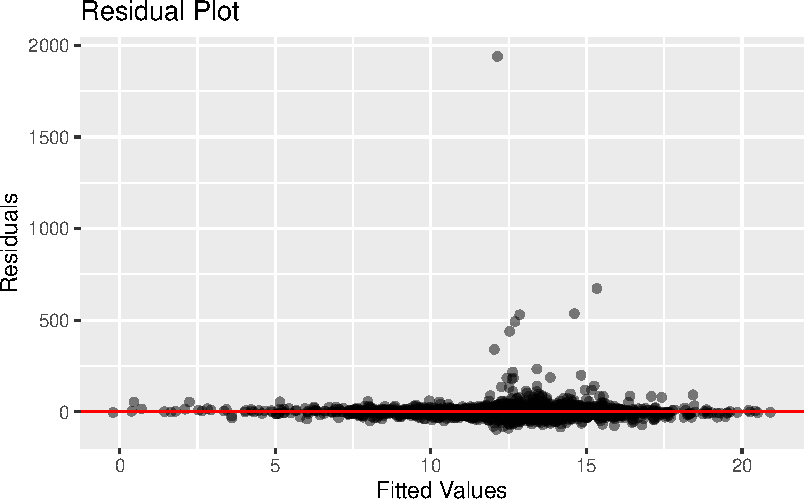
\includegraphics{draft_1_files/figure-pdf/unnamed-chunk-19-1.pdf}

\begin{Shaded}
\begin{Highlighting}[]
\CommentTok{\# Compare models by adjusted R{-}squared}
\NormalTok{model\_no\_new }\OtherTok{\textless{}{-}} \FunctionTok{lm}\NormalTok{(GrowthPercentage }\SpecialCharTok{\textasciitilde{}} \StringTok{\textasciigrave{}}\AttributeTok{GDP per capita}\StringTok{\textasciigrave{}} \SpecialCharTok{+} \StringTok{\textasciigrave{}}\AttributeTok{Value of global merchandise exports as a share of GDP}\StringTok{\textasciigrave{}}\NormalTok{, }\AttributeTok{data =}\NormalTok{ TradeData)}
\FunctionTok{summary}\NormalTok{(model\_no\_new)}\SpecialCharTok{$}\NormalTok{adj.r.squared}
\end{Highlighting}
\end{Shaded}

\begin{verbatim}
[1] 0.001264414
\end{verbatim}

\begin{Shaded}
\begin{Highlighting}[]
\FunctionTok{summary}\NormalTok{(model\_full)}\SpecialCharTok{$}\NormalTok{adj.r.squared}
\end{Highlighting}
\end{Shaded}

\begin{verbatim}
[1] 0.001091052
\end{verbatim}

\begin{Shaded}
\begin{Highlighting}[]
\CommentTok{\# Check for improvements in the model}
\ControlFlowTok{if}\NormalTok{ (}\FunctionTok{summary}\NormalTok{(model\_full)}\SpecialCharTok{$}\NormalTok{adj.r.squared }\SpecialCharTok{\textgreater{}} \FunctionTok{summary}\NormalTok{(model\_no\_new)}\SpecialCharTok{$}\NormalTok{adj.r.squared) \{}
  \FunctionTok{print}\NormalTok{(}\StringTok{"The new predictor improved the model."}\NormalTok{)}
\NormalTok{\} }\ControlFlowTok{else}\NormalTok{ \{}
  \FunctionTok{print}\NormalTok{(}\StringTok{"The new predictor did not improve the model."}\NormalTok{)}
\NormalTok{\}}
\end{Highlighting}
\end{Shaded}

\begin{verbatim}
[1] "The new predictor did not improve the model."
\end{verbatim}

The new predictor did not necessarily improve the model.

\textbf{\emph{We can now do some predictive model analysis}}

\begin{Shaded}
\begin{Highlighting}[]
\CommentTok{\# Run a linear model with all predictors including the new column}
\NormalTok{linear\_model\_full }\OtherTok{\textless{}{-}} \FunctionTok{lm}\NormalTok{(GrowthPercentage }\SpecialCharTok{\textasciitilde{}} \StringTok{\textasciigrave{}}\AttributeTok{GDP per capita}\StringTok{\textasciigrave{}} \SpecialCharTok{+} \StringTok{\textasciigrave{}}\AttributeTok{Value of global merchandise exports as a share of GDP}\StringTok{\textasciigrave{}} \SpecialCharTok{+}\NormalTok{ AnnualTradeValue, }\AttributeTok{data =}\NormalTok{ TradeData)}

\CommentTok{\# Add predictions to dataset}
\NormalTok{TradeData }\OtherTok{\textless{}{-}}\NormalTok{ TradeData }\SpecialCharTok{\%\textgreater{}\%}
  \FunctionTok{mutate}\NormalTok{(}\AttributeTok{PredictedGrowth =} \FunctionTok{predict}\NormalTok{(linear\_model\_full, }\AttributeTok{newdata =}\NormalTok{ TradeData))}

\CommentTok{\# Residual Analysis}
\FunctionTok{ggplot}\NormalTok{(TradeData, }\FunctionTok{aes}\NormalTok{(}\AttributeTok{x =}\NormalTok{ PredictedGrowth, }\AttributeTok{y =}\NormalTok{ GrowthPercentage }\SpecialCharTok{{-}}\NormalTok{ PredictedGrowth)) }\SpecialCharTok{+}
  \FunctionTok{geom\_point}\NormalTok{(}\AttributeTok{alpha =} \FloatTok{0.5}\NormalTok{) }\SpecialCharTok{+}
  \FunctionTok{geom\_hline}\NormalTok{(}\AttributeTok{yintercept =} \DecValTok{0}\NormalTok{, }\AttributeTok{color =} \StringTok{"red"}\NormalTok{) }\SpecialCharTok{+}
  \FunctionTok{labs}\NormalTok{(}
    \AttributeTok{title =} \StringTok{"Residual Analysis with New Predictor"}\NormalTok{,}
    \AttributeTok{x =} \StringTok{"Predicted Growth Percentage"}\NormalTok{,}
    \AttributeTok{y =} \StringTok{"Residuals"}
\NormalTok{  )}
\end{Highlighting}
\end{Shaded}

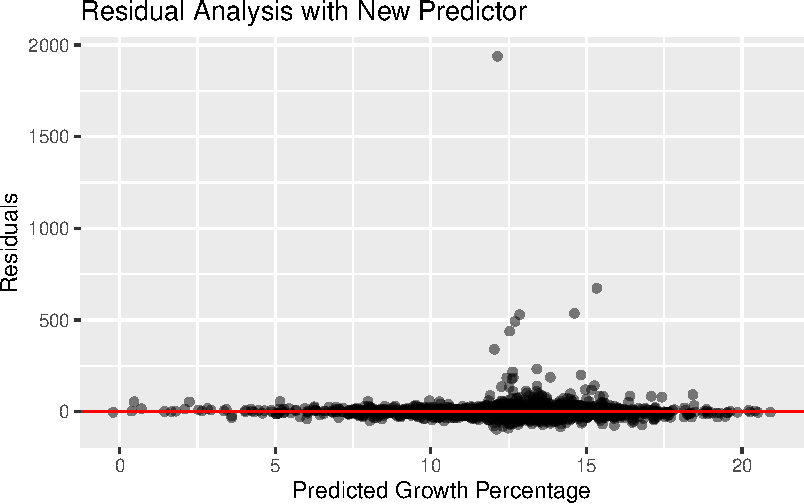
\includegraphics{draft_1_files/figure-pdf/unnamed-chunk-20-1.pdf}

\begin{Shaded}
\begin{Highlighting}[]
\NormalTok{model\_1 }\OtherTok{\textless{}{-}}\NormalTok{ model\_no\_new}
\NormalTok{model\_2 }\OtherTok{\textless{}{-}}\NormalTok{ model\_full}

\CommentTok{\# Model Summaries}
\FunctionTok{summary}\NormalTok{(model\_1)}
\end{Highlighting}
\end{Shaded}

\begin{verbatim}

Call:
lm(formula = GrowthPercentage ~ `GDP per capita` + `Value of global merchandise exports as a share of GDP`, 
    data = TradeData)

Residuals:
    Min      1Q  Median      3Q     Max 
 -96.22  -13.60   -3.25    7.90 1939.19 

Coefficients:
                                                          Estimate Std. Error
(Intercept)                                              1.205e+01  1.783e+00
`GDP per capita`                                        -1.252e-04  6.319e-05
`Value of global merchandise exports as a share of GDP`  8.094e-02  4.599e-02
                                                        t value Pr(>|t|)    
(Intercept)                                               6.756 1.74e-11 ***
`GDP per capita`                                         -1.982   0.0476 *  
`Value of global merchandise exports as a share of GDP`   1.760   0.0785 .  
---
Signif. codes:  0 '***' 0.001 '**' 0.01 '*' 0.05 '.' 0.1 ' ' 1

Residual standard error: 50.77 on 2677 degrees of freedom
Multiple R-squared:  0.00201,   Adjusted R-squared:  0.001264 
F-statistic: 2.696 on 2 and 2677 DF,  p-value: 0.06767
\end{verbatim}

\begin{Shaded}
\begin{Highlighting}[]
\FunctionTok{summary}\NormalTok{(model\_2)}
\end{Highlighting}
\end{Shaded}

\begin{verbatim}

Call:
lm(formula = GrowthPercentage ~ `GDP per capita` + `Value of global merchandise exports as a share of GDP` + 
    AnnualTradeValue, data = TradeData)

Residuals:
    Min      1Q  Median      3Q     Max 
 -96.41  -13.62   -3.18    7.89 1938.90 

Coefficients:
                                                          Estimate Std. Error
(Intercept)                                              1.213e+01  1.787e+00
`GDP per capita`                                        -1.058e-04  6.852e-05
`Value of global merchandise exports as a share of GDP`  7.814e-02  4.616e-02
AnnualTradeValue                                        -2.124e-09  2.903e-09
                                                        t value Pr(>|t|)    
(Intercept)                                               6.789 1.38e-11 ***
`GDP per capita`                                         -1.545   0.1225    
`Value of global merchandise exports as a share of GDP`   1.693   0.0906 .  
AnnualTradeValue                                         -0.732   0.4644    
---
Signif. codes:  0 '***' 0.001 '**' 0.01 '*' 0.05 '.' 0.1 ' ' 1

Residual standard error: 50.77 on 2676 degrees of freedom
Multiple R-squared:  0.00221,   Adjusted R-squared:  0.001091 
F-statistic: 1.975 on 3 and 2676 DF,  p-value: 0.1155
\end{verbatim}

\begin{Shaded}
\begin{Highlighting}[]
\NormalTok{TradeData\_country\_summary }\OtherTok{\textless{}{-}}\NormalTok{ TradeData }\SpecialCharTok{\%\textgreater{}\%}
  \FunctionTok{group\_by}\NormalTok{(CountryName) }\SpecialCharTok{\%\textgreater{}\%}
  \FunctionTok{summarise}\NormalTok{(}\AttributeTok{mean\_gdp\_per\_capita =} \FunctionTok{mean}\NormalTok{(}\StringTok{\textasciigrave{}}\AttributeTok{GDP per capita}\StringTok{\textasciigrave{}}\NormalTok{, }\AttributeTok{na.rm =} \ConstantTok{TRUE}\NormalTok{),}
            \AttributeTok{mean\_exports\_share\_of\_GDP =} \FunctionTok{mean}\NormalTok{(}\StringTok{\textasciigrave{}}\AttributeTok{Value of global merchandise exports as a share of GDP}\StringTok{\textasciigrave{}}\NormalTok{, }\AttributeTok{na.rm =} \ConstantTok{TRUE}\NormalTok{))}

\CommentTok{\# EDA Visualizations}
\CommentTok{\# Scatterplot: GDP per Capita vs. Exports}
\CommentTok{\# Exporting model summaries}
\NormalTok{broom}\SpecialCharTok{::}\FunctionTok{tidy}\NormalTok{(model\_1) }\SpecialCharTok{\%\textgreater{}\%} \FunctionTok{write.csv}\NormalTok{(}\StringTok{"Model\_1\_Summary.csv"}\NormalTok{)}
\NormalTok{broom}\SpecialCharTok{::}\FunctionTok{tidy}\NormalTok{(model\_2) }\SpecialCharTok{\%\textgreater{}\%} \FunctionTok{write.csv}\NormalTok{(}\StringTok{"Model\_2\_Summary.csv"}\NormalTok{)}


\CommentTok{\# Visualize GDP per capita vs exports share for different countries}
\FunctionTok{ggplot}\NormalTok{(TradeData\_country\_summary, }\FunctionTok{aes}\NormalTok{(}\AttributeTok{x =}\NormalTok{ mean\_gdp\_per\_capita, }\AttributeTok{y =}\NormalTok{ mean\_exports\_share\_of\_GDP)) }\SpecialCharTok{+}
  \FunctionTok{geom\_point}\NormalTok{() }\SpecialCharTok{+}
  \FunctionTok{labs}\NormalTok{(}\AttributeTok{title =} \StringTok{"Country{-}Level GDP vs Export Share of GDP"}\NormalTok{, }
       \AttributeTok{x =} \StringTok{"GDP per Capita"}\NormalTok{, }
       \AttributeTok{y =} \StringTok{"Exports as Share of GDP"}\NormalTok{) }\SpecialCharTok{+}
  \FunctionTok{theme\_minimal}\NormalTok{()}
\end{Highlighting}
\end{Shaded}

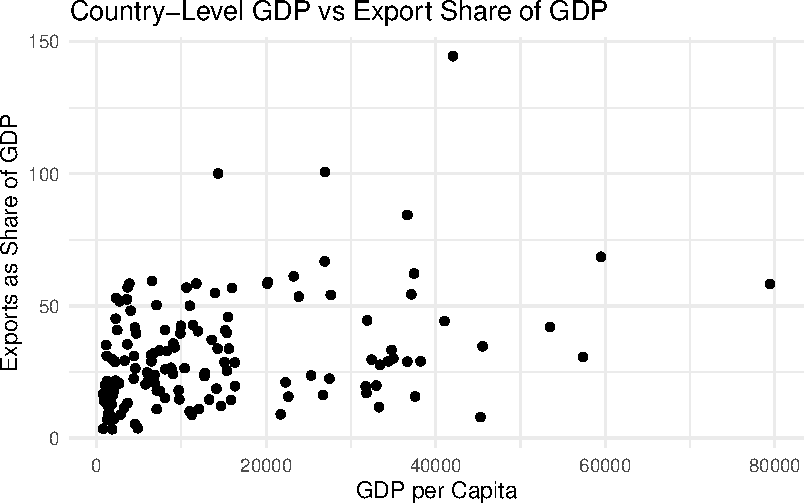
\includegraphics{draft_1_files/figure-pdf/unnamed-chunk-21-1.pdf}

\begin{Shaded}
\begin{Highlighting}[]
\CommentTok{\# Further statistical analysis: e.g., correlation between GDP per capita and export share}
\FunctionTok{cor}\NormalTok{(TradeData\_clean}\SpecialCharTok{$}\StringTok{\textasciigrave{}}\AttributeTok{GDP per capita}\StringTok{\textasciigrave{}}\NormalTok{, }
\NormalTok{    TradeData\_clean}\SpecialCharTok{$}\StringTok{\textasciigrave{}}\AttributeTok{Value of global merchandise exports as a share of GDP}\StringTok{\textasciigrave{}}\NormalTok{, }
    \AttributeTok{use =} \StringTok{"complete.obs"}\NormalTok{)}
\end{Highlighting}
\end{Shaded}

\begin{verbatim}
[1] 0.3067997
\end{verbatim}

\begin{Shaded}
\begin{Highlighting}[]
\CommentTok{\# For time series analysis, group by Year and summarize export share}
\NormalTok{TradeData\_year\_summary }\OtherTok{\textless{}{-}}\NormalTok{ TradeData\_clean }\SpecialCharTok{\%\textgreater{}\%}
  \FunctionTok{group\_by}\NormalTok{(Year) }\SpecialCharTok{\%\textgreater{}\%}
  \FunctionTok{summarise}\NormalTok{(}\AttributeTok{mean\_exports\_share\_of\_GDP =} \FunctionTok{mean}\NormalTok{(}\StringTok{\textasciigrave{}}\AttributeTok{Value of global merchandise exports as a share of GDP}\StringTok{\textasciigrave{}}\NormalTok{, }\AttributeTok{na.rm =} \ConstantTok{TRUE}\NormalTok{))}

\CommentTok{\# Plot export share over the years}
\FunctionTok{ggplot}\NormalTok{(TradeData\_year\_summary, }\FunctionTok{aes}\NormalTok{(}\AttributeTok{x =}\NormalTok{ Year, }\AttributeTok{y =}\NormalTok{ mean\_exports\_share\_of\_GDP)) }\SpecialCharTok{+}
  \FunctionTok{geom\_line}\NormalTok{(}\AttributeTok{color =} \StringTok{"red"}\NormalTok{) }\SpecialCharTok{+}
  \FunctionTok{labs}\NormalTok{(}\AttributeTok{title =} \StringTok{"Global Merchandise Exports as Share of GDP Over Time"}\NormalTok{, }
       \AttributeTok{x =} \StringTok{"Year"}\NormalTok{, }
       \AttributeTok{y =} \StringTok{"Mean Share of GDP"}\NormalTok{) }\SpecialCharTok{+}
  \FunctionTok{theme\_minimal}\NormalTok{()}
\end{Highlighting}
\end{Shaded}

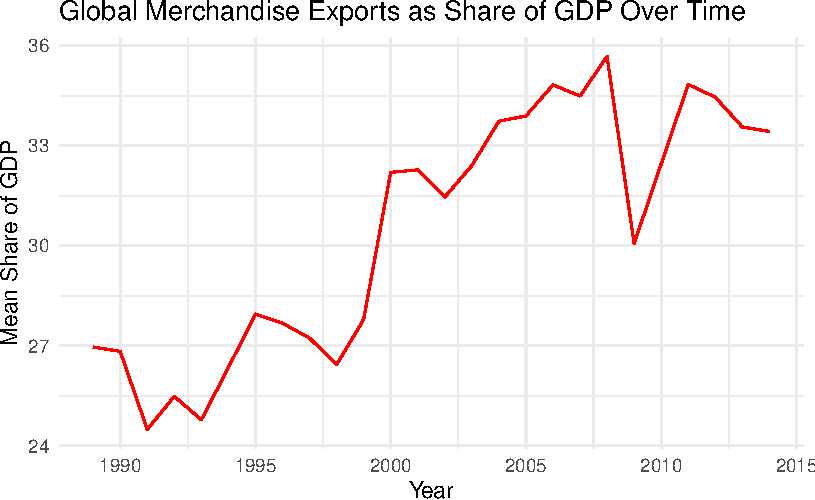
\includegraphics{draft_1_files/figure-pdf/unnamed-chunk-21-2.pdf}

\begin{Shaded}
\begin{Highlighting}[]
\CommentTok{\# Saving cleaned data for further analysis or export}
\FunctionTok{write\_csv}\NormalTok{(TradeData\_clean, }\StringTok{"cleaned\_data.csv"}\NormalTok{)}
\end{Highlighting}
\end{Shaded}

Both models suggest that the predictors
(\textbf{\texttt{GDP\ per\ capita}},
\textbf{\texttt{Value\ of\ global\ merchandise\ exports\ as\ a\ share\ of\ GDP}},
and \textbf{\texttt{AnnualTradeValue}}) explain very little of the
variation in growth percentage, as indicated by the low R-squared
values. Only the \textbf{\texttt{GDP\ per\ capita}} variable in the
first model is statistically significant at the 5\% level, with a
negative relationship to growth percentage. The export share of GDP has
a marginal significance (near the 10\% level) but does not show a strong
effect.

Thus, the models indicate weak explanatory power and suggest that other
factors not included in the model may have a stronger influence on
growth percentage.

\subsubsection{Advanced Analysis}\label{advanced-analysis}

\begin{Shaded}
\begin{Highlighting}[]
\CommentTok{\# Interaction terms in regression}
\NormalTok{model\_3 }\OtherTok{\textless{}{-}} \FunctionTok{lm}\NormalTok{(}\StringTok{\textasciigrave{}}\AttributeTok{Value of global merchandise exports as a share of GDP}\StringTok{\textasciigrave{}} \SpecialCharTok{\textasciitilde{}} 
              \StringTok{\textasciigrave{}}\AttributeTok{GDP per capita}\StringTok{\textasciigrave{}} \SpecialCharTok{*}\NormalTok{ GrowthPercentage, }\AttributeTok{data =}\NormalTok{ TradeData)}
\FunctionTok{summary}\NormalTok{(model\_3)}
\end{Highlighting}
\end{Shaded}

\begin{verbatim}

Call:
lm(formula = `Value of global merchandise exports as a share of GDP` ~ 
    `GDP per capita` * GrowthPercentage, data = TradeData)

Residuals:
    Min      1Q  Median      3Q     Max 
-41.887 -14.014  -5.579   9.059 138.749 

Coefficients:
                                   Estimate Std. Error t value Pr(>|t|)    
(Intercept)                       2.453e+01  6.207e-01  39.514   <2e-16 ***
`GDP per capita`                  4.097e-04  2.804e-05  14.614   <2e-16 ***
GrowthPercentage                  7.380e-05  1.549e-02   0.005    0.996    
`GDP per capita`:GrowthPercentage 1.037e-06  9.633e-07   1.077    0.282    
---
Signif. codes:  0 '***' 0.001 '**' 0.01 '*' 0.05 '.' 0.1 ' ' 1

Residual standard error: 21.32 on 2676 degrees of freedom
Multiple R-squared:  0.09556,   Adjusted R-squared:  0.09455 
F-statistic: 94.25 on 3 and 2676 DF,  p-value: < 2.2e-16
\end{verbatim}

\begin{Shaded}
\begin{Highlighting}[]
\CommentTok{\# Exporting interaction model summary}
\NormalTok{broom}\SpecialCharTok{::}\FunctionTok{tidy}\NormalTok{(model\_3) }\SpecialCharTok{\%\textgreater{}\%} \FunctionTok{write.csv}\NormalTok{(}\StringTok{"Model\_3\_Summary.csv"}\NormalTok{)}

\CommentTok{\# Feature Engineering}
\NormalTok{TradeData }\OtherTok{\textless{}{-}}\NormalTok{ TradeData }\SpecialCharTok{\%\textgreater{}\%}
  \FunctionTok{mutate}\NormalTok{(}
    \AttributeTok{Population\_in\_millions =}\NormalTok{ TradeData}\SpecialCharTok{$}\StringTok{"Population (historical)"} \SpecialCharTok{/} \FloatTok{1e6}\NormalTok{,}
    \AttributeTok{GDP\_to\_population\_ratio =} \StringTok{\textasciigrave{}}\AttributeTok{GDP per capita}\StringTok{\textasciigrave{}} \SpecialCharTok{/}\NormalTok{ TradeData}\SpecialCharTok{$}\StringTok{"Population (historical)"}
\NormalTok{  )}
\end{Highlighting}
\end{Shaded}

\begin{Shaded}
\begin{Highlighting}[]
\CommentTok{\# View the summarized country{-}level data}
\FunctionTok{head}\NormalTok{(TradeData\_country\_summary)}
\end{Highlighting}
\end{Shaded}

\begin{verbatim}
# A tibble: 6 x 3
  CountryName mean_gdp_per_capita mean_exports_share_of_GDP
  <chr>                     <dbl>                     <dbl>
1 Afghanistan               1828.                      3.33
2 Albania                   7080.                     11.0 
3 Algeria                   9055.                     35.8 
4 Angola                    7060.                     50.3 
5 Argentina                15829.                     14.4 
6 Armenia                   8044.                     15.2 
\end{verbatim}

\begin{Shaded}
\begin{Highlighting}[]
\CommentTok{\# Visualize GDP per capita vs exports share for different countries}
\FunctionTok{ggplot}\NormalTok{(TradeData\_country\_summary, }\FunctionTok{aes}\NormalTok{(}\AttributeTok{x =}\NormalTok{ mean\_gdp\_per\_capita, }\AttributeTok{y =}\NormalTok{ mean\_exports\_share\_of\_GDP)) }\SpecialCharTok{+}
  \FunctionTok{geom\_point}\NormalTok{() }\SpecialCharTok{+}
  \FunctionTok{labs}\NormalTok{(}\AttributeTok{title =} \StringTok{"Country{-}Level GDP vs Export Share of GDP"}\NormalTok{, }
       \AttributeTok{x =} \StringTok{"GDP per Capita"}\NormalTok{, }
       \AttributeTok{y =} \StringTok{"Exports as Share of GDP"}\NormalTok{) }\SpecialCharTok{+}
  \FunctionTok{theme\_minimal}\NormalTok{()}
\end{Highlighting}
\end{Shaded}

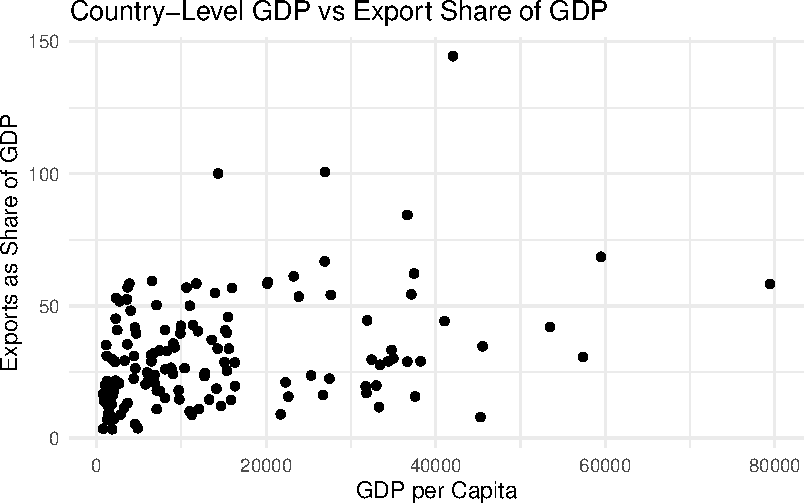
\includegraphics{draft_1_files/figure-pdf/unnamed-chunk-23-1.pdf}

\begin{Shaded}
\begin{Highlighting}[]
\CommentTok{\# Further statistical analysis: e.g., correlation between GDP per capita and export share}
\FunctionTok{cor}\NormalTok{(TradeData\_clean}\SpecialCharTok{$}\StringTok{\textasciigrave{}}\AttributeTok{GDP per capita}\StringTok{\textasciigrave{}}\NormalTok{, }
\NormalTok{    TradeData\_clean}\SpecialCharTok{$}\StringTok{\textasciigrave{}}\AttributeTok{Value of global merchandise exports as a share of GDP}\StringTok{\textasciigrave{}}\NormalTok{, }
    \AttributeTok{use =} \StringTok{"complete.obs"}\NormalTok{)}
\end{Highlighting}
\end{Shaded}

\begin{verbatim}
[1] 0.3067997
\end{verbatim}

\begin{Shaded}
\begin{Highlighting}[]
\CommentTok{\# For time series analysis, group by Year and summarize export share}
\NormalTok{TradeData\_year\_summary }\OtherTok{\textless{}{-}}\NormalTok{ TradeData\_clean }\SpecialCharTok{\%\textgreater{}\%}
  \FunctionTok{group\_by}\NormalTok{(Year) }\SpecialCharTok{\%\textgreater{}\%}
  \FunctionTok{summarise}\NormalTok{(}\AttributeTok{mean\_exports\_share\_of\_GDP =} \FunctionTok{mean}\NormalTok{(}\StringTok{\textasciigrave{}}\AttributeTok{Value of global merchandise exports as a share of GDP}\StringTok{\textasciigrave{}}\NormalTok{, }\AttributeTok{na.rm =} \ConstantTok{TRUE}\NormalTok{))}

\CommentTok{\# Plot export share over the years}
\FunctionTok{ggplot}\NormalTok{(TradeData\_year\_summary, }\FunctionTok{aes}\NormalTok{(}\AttributeTok{x =}\NormalTok{ Year, }\AttributeTok{y =}\NormalTok{ mean\_exports\_share\_of\_GDP)) }\SpecialCharTok{+}
  \FunctionTok{geom\_line}\NormalTok{(}\AttributeTok{color =} \StringTok{"red"}\NormalTok{) }\SpecialCharTok{+}
  \FunctionTok{labs}\NormalTok{(}\AttributeTok{title =} \StringTok{"Global Merchandise Exports as Share of GDP Over Time"}\NormalTok{, }
       \AttributeTok{x =} \StringTok{"Year"}\NormalTok{, }
       \AttributeTok{y =} \StringTok{"Mean Share of GDP"}\NormalTok{) }\SpecialCharTok{+}
  \FunctionTok{theme\_minimal}\NormalTok{()}
\end{Highlighting}
\end{Shaded}

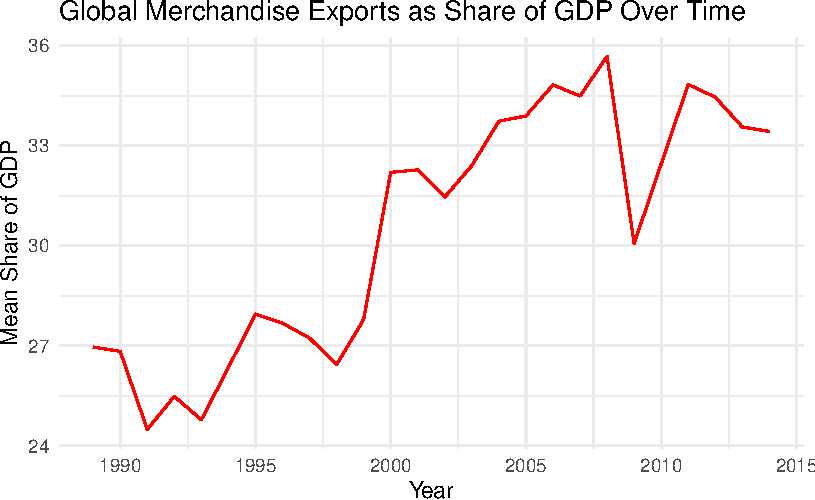
\includegraphics{draft_1_files/figure-pdf/unnamed-chunk-23-2.pdf}

\begin{Shaded}
\begin{Highlighting}[]
\CommentTok{\# Saving cleaned data for further analysis or export}
\FunctionTok{write\_csv}\NormalTok{(TradeData\_clean, }\StringTok{"cleaned\_data.csv"}\NormalTok{)}
\end{Highlighting}
\end{Shaded}





\end{document}
